\documentclass{beamer}
\usepackage{beamerthemesplit}
\usepackage{wrapfig}
\usetheme{SPbGU}
\usepackage{pdfpages}
\usepackage{amsmath}
\usepackage{mathtools}
\usepackage{cmap} 
\usepackage[T2A]{fontenc} 
\usepackage[utf8]{inputenc}
\usepackage[english,russian]{babel}
\usepackage{indentfirst}
\usepackage{amsmath}
\usepackage{tikz}
\usepackage{multirow}
\usepackage[noend]{algpseudocode}
\usepackage{algorithm}
\usepackage{algorithmicx}
\usepackage{ stmaryrd }
\usepackage{qtree}
\usetikzlibrary{shapes,arrows}
\usepackage{fancyvrb}
\newtheorem{rutheorem}{Теорема}
\newtheorem{ruproof}{Доказательство}
\newtheorem{rudefinition}{Определение}
\newtheorem{rulemma}{Лемма}
\beamertemplatenavigationsymbolsempty

\newcommand{\derive}[0]{\xRightarrow[]{*}}
\newcommand{\derivek}[1]{\xRightarrow[]{#1}}
\newcommand{\deriveg}[1]{\xRightarrow[#1]{*}}
\newcommand{\derivegone}[1]{\xRightarrow[#1]{}}

\title[]{Теория автоматов и формальных языков}
\subtitle[]{Контекстно-свободные языки}
\institute[]{
Санкт-Петербургский государственный электротехнический университет <<ЛЭТИ>>\\
}

\author[]{Екатерина Вербицкая}

\date{4 октября 2016г.}

\definecolor{orange}{RGB}{179,36,31}

\begin{document}
{
  \begin{frame}
    \titlepage
  \end{frame}
}


\begin{frame}[fragile]
  \transwipe[direction=90]
  \frametitle{В предыдущей серии}
  \begin{itemize}
    \item Регулярные выражения, регулярные грамматики и конечные автоматы задают класс регулярных языков
    \item Класс регулярных языков замкнут относительно теоретико-множественных операций, конкатенации, итерации, гомоморфизма цепочек
    \item Определение принадлежности слова языку осуществляется за $O(n)$ операций
    \item Однако класс регулярных языков достаточно узок, ни один используемый в промышленности язык программирования не является регулярным
    \begin{itemize}
      \item Лемма о накачке для доказательства нерегулярности языка
      \item Язык правильных скобочных последовательностей, язык палиндромов не являются регулярными
    \end{itemize}
  \end{itemize}
\end{frame}

\begin{frame}[fragile]
  \transwipe[direction=90]
  \frametitle{Контекстно-свободная грамматика}
  Четверка $\langle V_T, V_N, P, S \rangle$

   \begin{itemize}
     \item $V_T$ --- алфавит терминальных символов (терминалов) 
     \item $V_N$ --- алфавит нетерминальных символов (нетерминалов)
     \begin{itemize} 
        \item $V_T \cap V_N = \emptyset$ 
        \item $V ::= V_T \cup V_N$
     \end{itemize}
     \item P --- конечное множество правил вида $A \rightarrow \alpha$
     \begin{itemize}
       \item $A \in V_N $
       \item $\alpha \in V^*$
     \end{itemize}  
     \item S --- начальный нетерминал грамматики, $S  \in V_N$
  \end{itemize}

Пример: арифметические выражения

  $$
  \begin{array}{crcl}
  &E& \rightarrow & E + E \, | \, E * E \, | \, N \\
  &N& \rightarrow & 0 \, | \, 1  \, | \, \dots \, | \, 9
  \end{array}
  $$
\end{frame}

\begin{frame}[fragile]
  \transwipe[direction=90]
  \frametitle{Вывод в грамматике}
  \begin{itemize}
    \item \textbf{Отношение выводимости}: $\forall \alpha, \gamma, \delta \in V^*, A \in V_N: A \rightarrow \alpha \in P. \, \gamma A \delta \Rightarrow \gamma \alpha \delta$
    \item \textbf{Вывод} --- транизитивное, рефлексивное замыкание отношения выводимости ($\xRightarrow[]{*}, \xRightarrow[]{+}, \xRightarrow[]{k}$)
    \item \textbf{Левосторонний (правосторонний) вывод} --- на каждом шаге заменяем самый левый (правый) нетерминал
    \begin{itemize}
      \item Если не специфицируется, подразумевается левосторонний вывод
    \end{itemize}
    \item По сути, правила грамматики рассматриваются как правила переписывания
  \end{itemize}
\end{frame}

\begin{frame}[fragile]
  \transwipe[direction=90]
  \frametitle{Пример вывода}
  Построим левосторонний вывод цепочки $2+3*4$ в грамматике $\langle \{ 0, 1, \dots, 9, +, *\}, \{E, N\}, P, E \rangle$
  
  $$
  \begin{array}{crcl}
  &E& \rightarrow & E + N \, | \, E * N \, | \, N \\
  &N& \rightarrow & 0 \, | \, 1  \, | \, \dots \, | \, 9
  \end{array}
  $$
  
$E \Rightarrow  E * N \Rightarrow E + N * N \Rightarrow N + N * N \Rightarrow 2 + N * N \xRightarrow[]{2} 2 + 3 * 4$
\end{frame}

\begin{frame}[fragile]
  \transwipe[direction=90]
  \frametitle{Существование левостороннего вывода}
  \begin{rutheorem}
    Если для цепочки $\omega$ существует некоторый вывод $S \xRightarrow[]{*} \omega$, то существует и левосторонний вывод для этой цепочки $S \xRightarrow[l]{*} \omega$
  \end{rutheorem}
  \begin{proof}
  Докажем более общее утверждение: если существует $A \xRightarrow[]{*} \omega$, то существует $A \xRightarrow[l]{*} \omega$, где $A \in V_N$. 
  
  Доказываем по индукции по длине вывода $k$
  
    $k = 1: A \Rightarrow \omega$ --- тривиально. 
    
  $k \rightarrow k + 1: \sphericalangle A \Rightarrow \alpha \xRightarrow[]{*} \omega$. 
  
  Обозначим $ \alpha = B_1 B_2 \dots B_m \xRightarrow[]{*} \omega_1 \omega_2 \dots \omega_m = \omega; \forall i. B_i \xRightarrow[]{l_i} \omega_i, l_i \leq n$
  
  По индукционному предположению $\forall i. \, B_i \xRightarrow[l]{*} \omega_i$
  
  $\Mapsto: A \Rightarrow B_1 B_2 \dots B_m \xRightarrow[l]{*} \omega_1  B_2 \dots B_m \xRightarrow[l]{*} \omega$ --- левосторонний вывод
  \end{proof}
\end{frame}

\begin{frame}[fragile]
  \transwipe[direction=90]
  \frametitle{Единственность вывода}
  Не всегда (левосторонний) вывод единственен: 2 вывода строки $2+3*4$
  
  $$
  \begin{array}{crcl}
  &E& \rightarrow & E + E \, | \, E * E \, | \, N \\
  &N& \rightarrow & 0 \, | \, 1  \, | \, \dots \, | \, 9
  \end{array}
  $$

\begin{tabular}{p{5.5cm} p{6cm}}
  
\Tree [.E [.E [.N 2 ] ] + [.E [.E [.N 3 ] ] * [.E [.N 4 ] ] ] ] 
& 
\Tree [.E [.E [.E [.N 2  ] ]  + [.E [.N 3 ] ] ] * [.E [.N 4 ] ] ]  
\end{tabular}
\end{frame}

\begin{frame}[fragile]
  \transwipe[direction=90]
  \frametitle{Однозначность грамматики}
  \begin{itemize}
    \item Грамматика называется \textbf{однозначной}, если для \emph{любого} слова языка существует \emph{единственный} (левосторонний) вывод
    \item Грамматика называется \textbf{неоднозначной}, если \emph{существует} слово языка, такое что для него \emph{существует} \emph{несколько} (левосторонних) выводов
  \end{itemize}

  \begin{itemize}
    \item По однозначной грамматике можно тривиальным образом построить неоднозначную: продублировать правило
    \begin{itemize}
      \item $S \rightarrow A; A \rightarrow a$
      \item $S \rightarrow A | B; A \rightarrow a; B \rightarrow a$
     \end{itemize}
     \item Не существует общего алгоритма преобразования неоднозначной грамматики в однозначную
   \end{itemize}
\end{frame}

\begin{frame}[fragile]
  \transwipe[direction=90]
  \frametitle{Примеры однозначной и неоднозначной грамматики}
  \begin{itemize}
    \item { Неоднозначная грамматика
  $$
  \begin{array}{crcl}
  &E& \rightarrow & E + E \, | \, E * E \, | \, N \\
  &N& \rightarrow & 0 \, | \, 1  \, | \, \dots \, | \, 9
  \end{array}
  $$
  }
    \item { Однозначная грамматика
  $$
  \begin{array}{crcl}
  &E& \rightarrow & E + N \, | \, E * N \, | \, N \\
  &N& \rightarrow & 0 \, | \, 1  \, | \, \dots \, | \, 9
  \end{array}
  $$
  }
  \end{itemize}
\end{frame}

\begin{frame}[fragile]
  \transwipe[direction=90]
  \frametitle{Проверка однозначности грамматики --- неразрешимая задача}
  \begin{itemize}
    \item Проверка однозначности грамматик сводится к задаче соответствий Поста
  \end{itemize}
    \begin{itemize}
    \item Задача соответствий Поста: Даны списки $A = (a_1, \dots, a_n)$ и $B = (b_1 ,\dots ,b_n)$, где $\forall i. \, a_i \in \Sigma ^*$ и $b_i \in \Sigma ^*$.Cуществует ли непустая последовательность $(i_1 , \dots, i_k)$, удовлетворяющая условию $a_{i_1} \dots a_{i_k} = b_{i_1} \dots b_{i_k}$, где $\forall j. \, 1 \leq i_j \leq n$
  \end{itemize}
\end{frame}


\begin{frame}[fragile]
  \transwipe[direction=90]
  \frametitle{Контекстно-свободный язык}
  \begin{itemize}
    \item Язык называется \textbf{контекстно-свободным}, если для него \emph{существует} контекстно-свободная грамматика
    \item Язык, задаваемый КС грамматикой $\langle V_T, V_N, P, S\rangle$: $\{ \omega \in V_T^* | S \xRightarrow[]{*} \omega \}$
    \item КС язык называется \textbf{существенно неоднозначным}, если для него не существует однозначной грамматики
  \end{itemize}
\end{frame}


\begin{frame}[fragile]
  \transwipe[direction=90]
  \frametitle{Пустота КС языка}
   \begin{rutheorem}
   Существует алгоритм, определяющий, является ли язык, порождаемый КС грамматикой, пустым
   \end{rutheorem}
   \begin{proof}
     Для доказательства потребуется следующая лемма
   \end{proof}
\end{frame}
  
\begin{frame}[fragile]
  \transwipe[direction=90]
  \frametitle{Лемма}
   \begin{rutheorem}
   Если в данной грамматике выводится некоторая цепочка, то существует цепочка, дерево вывода которой не содержит ветвей длиннее $m$, где $m$ --- количество нетерминалов грамматики
   \end{rutheorem}
   \begin{proof}
   Рассмотрим дерево вывода цепочки $\omega$. Если в нем есть 2 узла, соответствующих одному нетерминалу $A$, обозначим их $n_1$ и $n_2$. Предположим, $n_1$ расположен ближе к корню дерева, чем $n_2$; $A_{n_1} \xRightarrow[]{*} \alpha \omega_1 \beta; A_{n_2} \xRightarrow[]{*} \gamma \omega_2 \delta$. При этом $\omega_2$ является подцепочкой $\omega_1$. 
   
   Заменим в изначальном дереве узел $n_1$ на $n_2$. Полученное дерево является деревом вывода $\alpha \omega_2 \delta$. Повторяем процесс замены одинаковых нетерминалов до тех пор, пока в дереве не останутся только уникальные нетерминалы. 
   
   В полученном дереве не может быть ветвей длины большей, чем $m$. По постороению оно является деревом вывода. 
   \end{proof}
\end{frame}

\begin{frame}[fragile]
  \transwipe[direction=90]
  \frametitle{Алгоритм проверки пустоты КС языка}
   \begin{proof}
   Строим коллекцию деревьев, представляющих вывод в грамматике.
   
  \begin{enumerate}
    \item Инициализируем коллекцию деревом из одного узла S
    \item Добавляем в коллекцию дерево, полученное применением единственного правила грамматики из какого-нибудь дерева из коллекции, если его в нем еще нет, и самая длинная ветвь не длиннее $m$
    \item Если после окончания построения коллекции в ней существует дерево, являющееся деревом вывода некоторой цепочки терминалов, значит, язык не пуст
  \end{enumerate}
   \end{proof}
\end{frame}

\begin{frame}[fragile]
  \transwipe[direction=90]
  \frametitle{Упрощение КС грамматики: удаление непродуктивных нетерминалов}
  \textbf{Продуктивный нетерминал}:  нетерминал, для которого существует цепочка терминалов, выводимая из него ($\exists \omega \in V_T^*. \, A \xRightarrow[]{*} \omega$)

  \textbf{Непродуктивный нетерминал}:  нетерминал, не являющийся продуктивным
\end{frame}

\begin{frame}[fragile]
  \transwipe[direction=90]
  \frametitle{Упрощение КС грамматики: удаление непродуктивных нетерминалов}

  \begin{rutheorem}
    Для любой КС грамматики $G = \langle V_T, V_N, P, S\rangle: L(G) \neq \varnothing$, можно постороить эквивалентную грамматику, каждый нетерминал которой продуктивен
  \end{rutheorem}

   \begin{proof}
   Удаляем из грамматики все нетерминалы $A: L(A) = \varnothing$, а также правила, использующие их. Полученную грамматику обозначаем $G_1$.

   Докажем, что $L(G) = L(G_1)$. Очевидно, $L(G_1) \subseteq L(G)$.

   Докажем от противного, что $L(G) \subseteq L(G_1)$. Предположим, что $\exists \omega \in L(G)$, но $\omega \notin L(G_1)$. 
   Тогда $S \xRightarrow[]{*} \alpha_1 A \alpha_2 \xRightarrow[]{*} \omega$, где $A \in V_N \setminus V_{N_1}$, но тогда $\exists \gamma \in V_T^*. \, A \xRightarrow[]{*} \gamma $. Противоречие
   \end{proof}
\end{frame}

\begin{frame}[fragile]
  \transwipe[direction=90]
  \frametitle{Упрощение КС грамматики: приведение}

  \begin{rutheorem}
    Для любой КС грамматики, порождающей непустой язык, можно постороить эквивалентную, для каждого нетерминала $A$ которой существует вывод вида $S \derive \omega_1 A \omega_3 \derive \omega_1 \omega_2 \omega_3, \omega_i \in V_T^*$
  \end{rutheorem}

   \begin{proof}
   Будем рассматривать грамматику без непродуктивных нетерминалов $G_1 = \langle V_{N_1}, V_T, P_1, S\rangle$.
   
   Верно: если существует $S \derive \alpha_1 A \alpha_3, \alpha_i \in V^*$, то $S \derive \alpha_1 A \alpha_3 \derive \omega_1 A \omega_3 \derive \omega_1 \omega_2 \omega_3, \omega_i \in V_T^*$
   
   Строим множество нетерминалов, встречающихся в выводах: добавляем сначала $S$, потом добавляем нетерминалы, встречающиеся в правой части правил для нетерминалов из множества. Завершаем процесс, когда больше ничего не добавить. Обозначаем полученное множество $V_{N_2}$, удаляем все правила грамматики, содержащие нетерминалы из $ V_{N_1} \setminus V_{N_2}$
   
   
   \end{proof}
\end{frame}

\begin{frame}[fragile]
  \transwipe[direction=90]
  \frametitle{Упрощение КС грамматики: приведение}
   \begin{proof}
   Получили грамматику $G_2 = \langle V_{N_2}, V_T, P_2, S\rangle$. 

   Докажем: $L(G_2) = L(G_1)$
   
   $L(G_2) \subseteq L(G_1)$, так как $P_2 \subseteq P_1$
   
   Докажем: $L(G_1) \subseteq L(G_2)$. Пусть $S \deriveg{G_1} \omega$. Все нетерминалы, встречающиеся в этом выводе содержатся в $V_{N_2}$, соответственно используются только правила из $ P_2 \Rightarrow S \deriveg{G_2} \omega $
   
   Так как все нетерминалы $V_{N_2}$ продуктивны, то  $S \derive \omega_1 A \omega_3 \derive \omega_1 \omega_2 \omega_3, \omega_i \in V_T^*$
   
   
   \end{proof}
   
   Грамматика $G_2$ называется \textbf{приведенной}, ее нетерминалы --- \textbf{достижимыми}
   
   Недостижимые и непродуктивные нетерминалы называются \textbf{бесполезными}
\end{frame}

\begin{frame}[fragile]
  \transwipe[direction=90]
  \frametitle{Упрощение КС грамматики: удаление цепных правил}
  Правило называется \textbf{цепным}, если оно имеет вид $A \rightarrow B; A, B \in V_N$.
  
  \begin{rutheorem}
    Для любой КС грамматики $G=\langle V_N, V_T, P, S \rangle$ можно построить эквивалентную, не содержащую цепных правил
  \end{rutheorem}
  
   \begin{proof}
   Строим новое множество правил $P_1$. Включаем в него все нецепные правила  $P$. Затем добавляем в $P_1$ правила вида $A \derive \alpha$, если $A \derive B$, где $A, B \in V_N$ и $B \rightarrow \alpha$ --- нецепное правило из $P$.
   
   Замечание: достаточно проверять только цепные выводы длины меньшей, чем $V_N$
   
   Обозначим полученную грамматику за $G_1=\langle V_N, V_T, P_1, S \rangle$, докажем $L(G_1)=L(G)$
      \end{proof}
\end{frame} 
   
\begin{frame}[fragile]
  \transwipe[direction=90]
  \frametitle{Упрощение КС грамматики: удаление цепных правил}    
  \begin{proof}   
   Очевидно $L(G_1) \subseteq L(G)$
   
   Покажем $L(G) \subseteq L(G_1)$. Пусть $\omega \in L(G)$. Рассмотрим левосторонний вывод $S \derivegone{G} \alpha_0 \derivegone{G} \alpha_1 \derivegone{G} \dots \derivegone{G} \alpha_n = \omega$.
   
   Предположим $\alpha_i \derivegone{G} \alpha_{i+1}$ --- первый шаг, выполняемый посредством цепного правила в выводе; $\forall k \in [i..j]. \, \alpha_k \derivegone{G} \alpha_{k+1}$ --- посредством цепного правила;  $\alpha_j \derivegone{G} \alpha_{j+1}$  --- посредством нецепного правила
   
   Тогда $|\alpha_i| = |\alpha_{i+1}| = \dots = |\alpha_j|$, и на каждом шаге заменяется один и тот же нетерминал. Тогда $\alpha_i \derivegone{G_1} \alpha_{j+1} $ посредством правила из $P_1 \setminus P \Rightarrow \omega \in L(G_1)$
   \end{proof}
   
\end{frame}

 
\begin{frame}[fragile]
  \transwipe[direction=90]
  \frametitle{Нормальная форма Хомского}    
  КС грамматика находится в \textbf{нормальной форме Хомского}, если все ее правила имеют вид $A \rightarrow B C$, или $A \rightarrow a$, где $A,B,C \in V_N, a \in V_T$
  
  \begin{rutheorem}   
    Для любой КС грамматики можно построить эквивалентную в нормальной форме Хомского
  \end{rutheorem}

     \begin{enumerate}
    \item Удаляем цепные правила. Теперь $\forall A \rightarrow B. \, B \in V_T$
    \item Заменяем правило $A \rightarrow B_1 B_2 \dots B_n$ на $A \rightarrow C_1 C_2 \dots C_n$, где $C_i = B_i,$ если $B_i \in V_N$, или $C_i \rightarrow B_i$, если $B_i \in V_T$
    \item Заменяем правило $A \rightarrow C_1 C_2 \dots C_n$ на множество правил $A \rightarrow C_1 D1, D1 \rightarrow C_2 D_2, \dots, D_{n-3} \rightarrow C_{n-2} D_{n-2}, D_{n-2} \rightarrow C_{n-1} C_n$
  \end{enumerate}
  
        Полученная грамматика находится в НФХ и эквивалентна данной 
\end{frame}

\begin{frame}[fragile]
  \transwipe[direction=90]
  \frametitle{Пример приведения в НФХ}    
  $G = \langle \{S, A, B\}, \{a, b\}, P, S\rangle$, где P:
  
  $$
  \begin{array}{crclllll}
   & S & \rightarrow & bA &\, | \, & aB \\
   & A & \rightarrow & a &\, | \, & aS &\, | \,&  bAA  \\
   & B & \rightarrow &  b & \, | \, &  bS & \, | \, & a BB 
  \end{array}
  $$
  
  \begin{itemize}
    \item $S \rightarrow b A \Mapsto S \rightarrow C_1 A; C_1 \rightarrow b$
    \item $S \rightarrow a B \Mapsto S \rightarrow C_2 B; C_2 \rightarrow a$
    \item $A \rightarrow aS \Mapsto A \rightarrow C_3 S; C_3 \rightarrow a$
    \item $A \rightarrow b A A \Mapsto A \rightarrow C_4 D_1; C_4 \rightarrow b; D_1 \rightarrow A A$
    \item $B \rightarrow b S \Mapsto B \rightarrow C_5 S; C_5 \rightarrow b$
    \item $B \rightarrow a B B \Mapsto B \rightarrow C_6 D_2; C_6 \rightarrow a; D_2 \rightarrow B B$
  \end{itemize}
\end{frame}


\begin{frame}[fragile]
  \transwipe[direction=90]
  \frametitle{Еще немного упростим}      
  
    $$
  \begin{array}{crclllll}
   & S & \rightarrow & bA &\, | \, & aB \\
   & A & \rightarrow & a &\, | \, & aS &\, | \,&  bAA  \\
   & B & \rightarrow &  b & \, | \, &  bS & \, | \, & a BB 
  \end{array}
  $$
  
  ~\\~
  
  $$
  \begin{array}{crclllll}
   & S & \rightarrow & C_b A &\, | \, & C_a B \\
   & A & \rightarrow & a &\, | \, & C_a S &\, | \,&  C_b D_1  \\
   & B & \rightarrow &  b & \, | \, &  C_b S & \, | \, & C_a D_2 \\
   & D_1 & \rightarrow & A A & \\
   & D_2 & \rightarrow & B B & \\
   & C_a & \rightarrow & a & \\
   & C_b & \rightarrow & b & 
  \end{array}
  $$
  
\end{frame}

\begin{frame}[fragile]
  \transwipe[direction=90]
  \frametitle{Алгоритм приведения в НФХ}      
  
  \begin{enumerate}
    \item Удалить стартовый нетерминал из правых частей правил 
    \begin{itemize}
      \item добавляется новое правило $S_0 \rightarrow S, S_0 \notin V_N, S_0$ делается новым стартовым
    \end{itemize}
    \item Избавиться от неодиночных терминалов в правых частях 
    \begin{itemize} 
      \item новое правило $C_c \rightarrow c$
    \end{itemize}
    \item Удалить длинные правила (длины больше 2)
    \item Удалить непродуктивные правила ($\varepsilon$-правила)
    \begin{itemize}
      \item Если $A \rightarrow \varepsilon$, то $A$ --- $\varepsilon$-правило
      \item Если $A \rightarrow X_1 X_2 \dots X_n, \forall i. \, X_i$ --- $\varepsilon$-правило, то $A$ --- $\varepsilon$-правило
      \item Заменяем $A \rightarrow X_1 X_2 \dots X_n$ на множество правил, где каждое из $\varepsilon$-правил опущено во всех возможных комбинациях, удаляем те, которые выводят $\varepsilon$
    \end{itemize}
    \item Удалить цепные правила
    \begin{itemize}
      \item Для каждой пары правил $A \rightarrow B; B \rightarrow  X_1 X_2 \dots X_n$ добавить правило $A \rightarrow  X_1 X_2 \dots X_n$, цепное правило удалить
    \end{itemize}
  \end{enumerate}
\end{frame}

\begin{frame}[fragile]
  \transwipe[direction=90]
  \frametitle{Порядок действий при приведении в НФХ}      
  Порядок \textbf{важен}!
  
  \begin{enumerate}
    \item Удалить стартовый нетерминал из правых частей правил 
    \item Избавиться от неодиночных терминалов в правых частях 
    \item Удалить длинные правила (длины больше 2)
    \item Удалить непродуктивные правила ($\varepsilon$-правила)
    \item Удалить цепные правила
  \end{enumerate}

  \begin{itemize}
    \item 1 шаг порождает новые цепные правила, поэтому его нельзя выполнять после 5 шага
    \item Если выполнить 4 шаг перед 3 шагом, то произойдет экспоненциальный взрыв грамматики
    \item 5 шаг приводит к квадратичному возрастанию размера грамматики
    \item Наиболее эффективны порядки $1, 2, 3, 4, 5$ и $1,3, 4,5,2$
  \end{itemize}
\end{frame}

\begin{frame}[fragile]
  \transwipe[direction=90]
  \frametitle{Увеличение размера грамматики при нормализации}      
  Порядок \textbf{важен}!
  
  \begin{enumerate}
    \item Удалить стартовый нетерминал из правых частей правил 
    \begin{itemize}
      \item Увеличение на 1
    \end{itemize}
    \item Избавиться от неодиночных терминалов в правых частях 
    \begin{itemize}
      \item Увеличение на $|V_T|$ правил
    \end{itemize}
    \item Удалить длинные правила (длины больше 2)
    \begin{itemize}
      \item Увеличение не более, чем в 2 раза (для правил длины $k \geq 3$ порождается $k-1$ новых правил)
    \end{itemize}
    \item Удалить непродуктивные правила ($\varepsilon$-правила)
    \begin{itemize}
      \item Увеличение не более, чем в 3 раза
    \end{itemize}
    \item Удалить цепные правила
    \begin{itemize}
      \item Увеличение не более, чем в $O(n^2)$ (цепных правил не больше $n^2$, где $n$ --- число нетерминалов)
    \end{itemize}
  \end{enumerate}
  
  Итого: \textbf{полиномиальное} увеличение размеров грамматики при правильном порядке действий
\end{frame}

\begin{frame}[fragile]
  \transwipe[direction=90]
  \frametitle{Синтаксический анализ: алгоритм Кока-Янгера-Касами (Cocke-Younger-Kasami algorithm, CYK)}
  Что значит $A \rightarrow a$? \pause
  
  ~\\~
  
 $A \Rightarrow a  \derive \omega \Leftrightarrow \omega = a$ 
\end{frame}

\begin{frame}[fragile]
  \transwipe[direction=90]
  \frametitle{Синтаксический анализ: алгоритм Кока-Янгера-Касами (Cocke-Younger-Kasami algorithm)}
  Что значит $A \rightarrow BC$? \pause
  
  ~\\~
  
  $A \Rightarrow BC  \derive \omega \Leftrightarrow \exists \omega_1, \omega_2 . \, \omega = \omega_1 \omega_2; B \derive \omega_1; C \derive \omega_2$ \pause
  
  ~\\~
  
  Или $A \Rightarrow BC  \derive \omega \Leftrightarrow \exists k \in [1 \dots |\omega|]. \,  B \derive \omega[1\dots k]; C \derive \omega[k+1 \dots |\omega|]$
\end{frame}

\begin{frame}[fragile]
  \transwipe[direction=90]
  \frametitle{Синтаксический анализ: алгоритм Кока-Янгера-Касами (Cocke-Younger-Kasami algorithm, CYK)}
  \begin{itemize}
      \item Алгоритм синтаксического анализа, работающий с грамматиками в НФХ
      \item Динамическое программирование
  \end{itemize}

  \begin{center}
    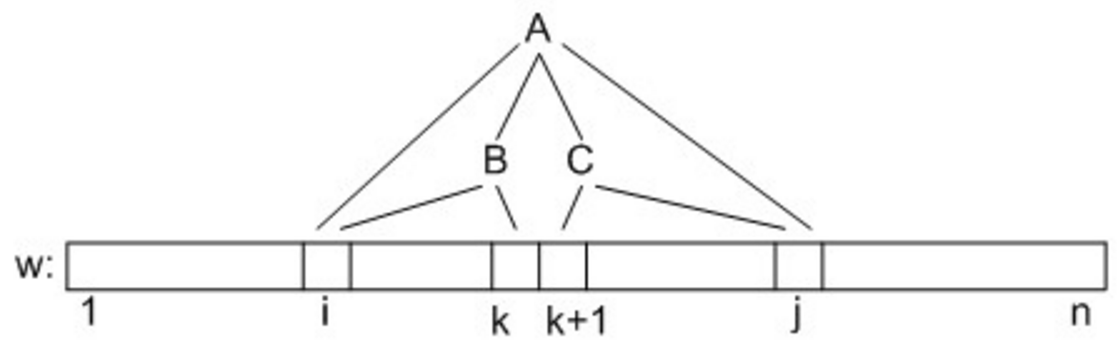
\includegraphics[width=\textwidth]{pics/CYK.png}  
  \end{center}
\end{frame}


\begin{frame}[fragile]
  \transwipe[direction=90]
  \frametitle{CYK}
  \begin{itemize}
      \item Дано: строка $\omega$ длины $n$, грамматика $G = \langle V_T, V_N, P, S\rangle$ в НФХ
      \item Используем трехмерный массив d булевых значений размером $|V_N| \times n \times n$, $d[A][i][j] = true \Leftrightarrow A \derive \omega[i \dots j]$
      \item Инициализация: $i = j$
      \begin{itemize}
        \item $d[A][i][i] = true$, если в грамматике есть правило $A \rightarrow \omega[i]$
        \item $d[A][i][i] = false$, иначе
      \end{itemize}
      \item Динамика. Предполагаем, d построен для всех нетерминалов и пар $\{(i', j') \, | \, j' - i' < m \}$
      \begin{itemize}
        \item $d[A][i][j] = \bigvee_{A\rightarrow BC}^{}{\bigvee_{k=i}^{j-1}{d[B][i][k] \wedge d[C][k][j]}}$
      \end{itemize}
      \item В конце работы алгоритма в $d[S][0][n]$ записан ответ, выводится ли $\omega$ в данной грамматике
  \end{itemize}
\end{frame}

 \end{document}
 

  
